\documentclass{article}

\usepackage{graphicx}
\usepackage[hidelinks]{hyperref}
\usepackage{geometry}
\usepackage{amsmath}
\usepackage{listings}
\usepackage{wrapfig}
\usepackage{mwe}

\geometry{
 a4paper,
 left=20mm,
 right=20mm,
 top=20mm,
 bottom=25mm,
}

\begin{document}

\begin{titlepage}
\begin{center}
\vspace*{1cm}
            
\Huge
\textbf{Assignment 1}
            
\vspace{1cm}

\Large
\text{Tuesday, September 17, 2024}

\vspace{2cm}

\text{\texttt{Jeremy Middleman}} \\
\text{\texttt{Andrei Phelps}} \\
\text{\texttt{Wayne Rudnick}} \\
\text{\texttt{Brian}} \\
\text{\texttt{Thomas Hynes}} \\

\vspace{2cm}

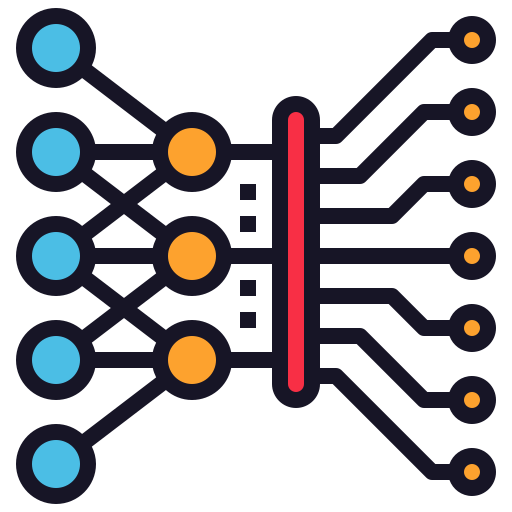
\includegraphics[scale=0.25]{../figs/icon.png}\\[0.5cm]

\vspace{9cm}

\textbf{CS 491: Neural Network} \\

\end{center}
\end{titlepage}

\newpage

\section{Individual Contributions}
\subsection{Wayne Rudnick}
1) Initialized the github repository and helped everyone start on the project. \\
2) Part 1 - created the python class for perceptions.\\
3) Part 2 - created the fit function in the perception class for perceptron learning.\\
4) Part 3 - Created the test cases and used the training data I generated to train the perceptron. Then ploted the data and the separation hyperplane. Printed the number of misclassified training samples in the console.\\
5) Helped to oversee and assist with parts 4 and 5. Passed over my code from previous parts and explained/helped modify it to fit the desired reslut for the new parts.
6) Generated the tests for parts 1-3 and graphed for different number of epochs, samples, etc.




\section{Perceptron}


\subsection{100 Samples}

For parts 1-3 of the assignment, we chose to run our test with a learning rate of 0.1 and with 10 epochs. In this test, we saw that the perceptron was able to correctly classify all samples for case #1 and missed 5 samples for case #2. Even with this relatively low number of ephocs, we were impressed with how well the perceptron did classifying the data.

\begin{center}
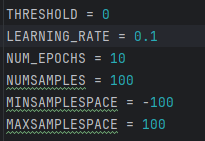
\includegraphics[scale=0.75]{../figs/P1.1.png}\\
\end{center}

\begin{center}
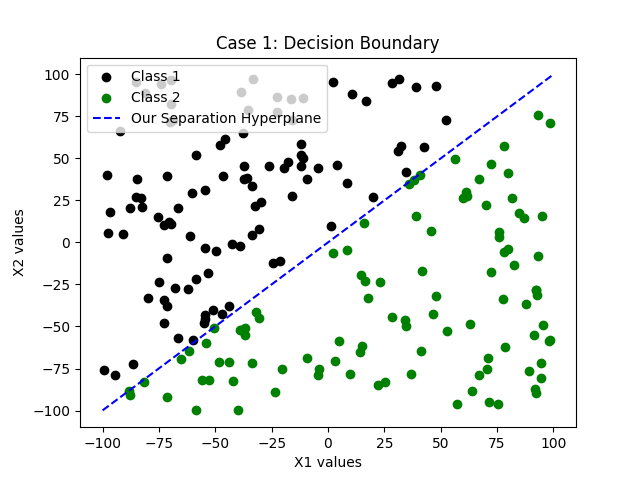
\includegraphics[scale=0.75]{../figs/P1.2.png}\\
\end{center}

\begin{center}
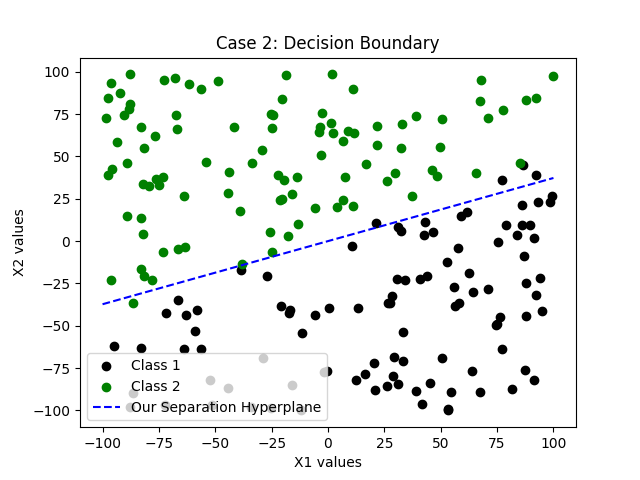
\includegraphics[scale=0.75]{../figs/P1.3.png}\\
\end{center}

\begin{center}
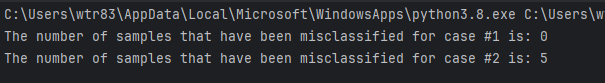
\includegraphics[scale=0.75]{../figs/P1.4.png}\\
\end{center}

\subsection{10,000 Samples}

For our additional test with 10,000 samples we observed a very defining line between class 1 and class 2. We wanted to include this test in our document because we believe it does a good job of showing how well the separation hyperplane is positioned when it has lots of training data. In this example, the hyperplane only has a mistake rate of approximately 1%.

\begin{center}
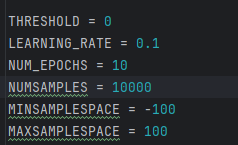
\includegraphics[scale=0.75]{../figs/P2.1.png}\\
\end{center}

\begin{center}
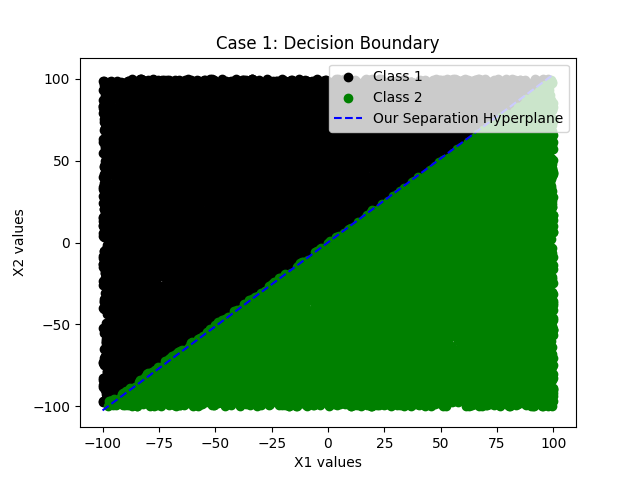
\includegraphics[scale=0.75]{../figs/P2.2.png}\\
\end{center}

\begin{center}
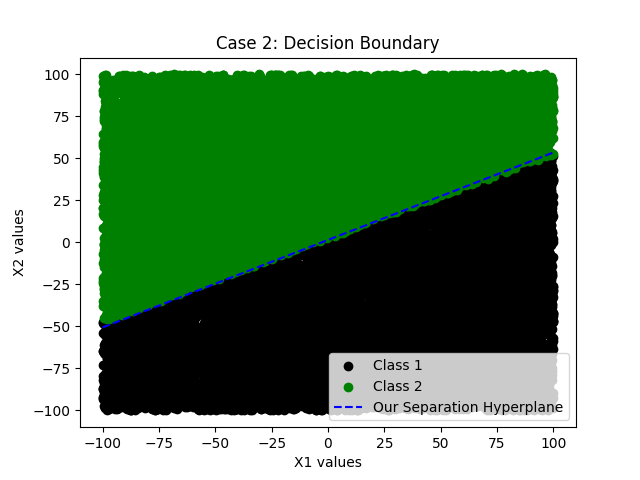
\includegraphics[scale=0.75]{../figs/P2.3.png}\\
\end{center}

\begin{center}
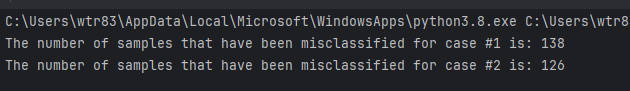
\includegraphics[scale=0.75]{../figs/P2.4.png}\\
\end{center}

\section{Gradient Descent}

For parts 4-5 of the assignment... (general overview).

\begin{center}
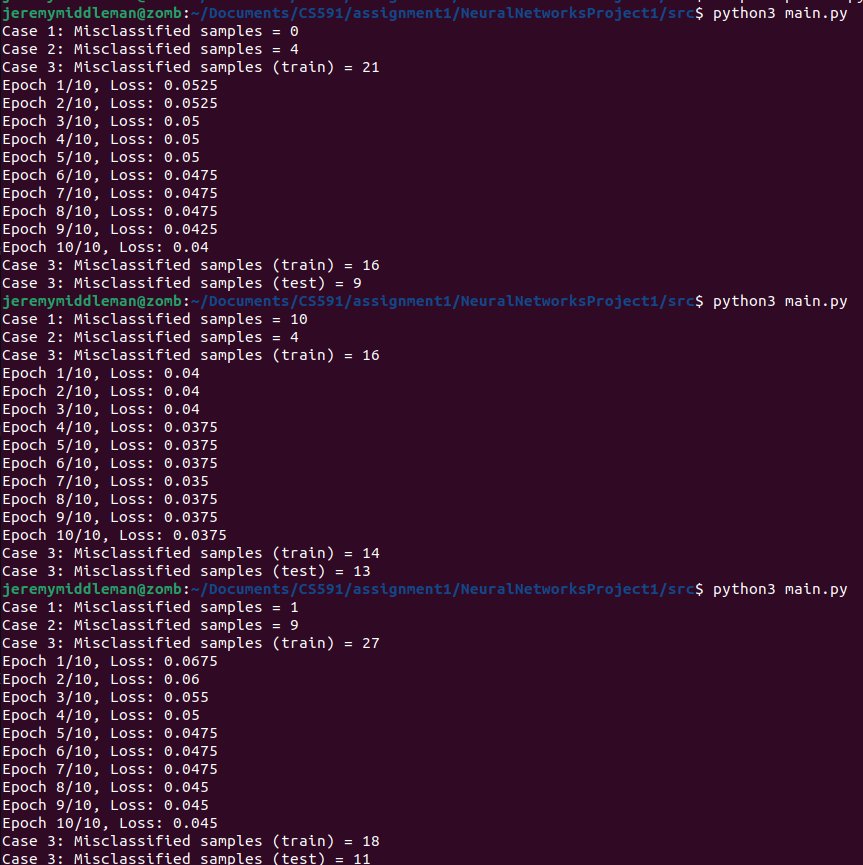
\includegraphics[scale=0.5]{../figs/P3.1.png}\\
\end{center}

\end{document}
